% !TEX TS-program = pdflatex
% !TEX encoding = UTF-8 Unicode

% TeX-M (r1.1)
% For my math classes at UT Austin
% Notes template created by Abdon Morales for the College of Natural Science
% and for the Department of Mathematics and Computer Science
% (c) 2019 - 2024 Abdon Morales and the University of Texas at Austin
% This is a notes template for a LaTeX document using the "article" class for Mathematics (Calculus)
% at the University of Texas at Austin.

% Last change made: Jan 27, 2024 1:40 AM CST

% See "book", "report", "letter" for other types of document.

\documentclass[11pt]{article} % use larger type; default would be 10pt

% Start of Article customization options and addons (for more help and information reference to Overleaf's guides and docs on Latex.
\usepackage[utf8]{inputenc} % set input encoding (not needed with XeLaTeX)

%%% Examples of Article customizations
% These packages are optional, depending whether you want the features they provide.
% See the LaTeX Companion or other references for full information.

%%% PAGE DIMENSIONS
\usepackage{geometry} % to change the page dimensions
\geometry{letterpaper} % or letterpaper (US) or a5paper or....
% \geometry{margin=2in} % for example, change the margins to 2 inches all round
% \geometry{landscape} % set up the page for landscape
%   read geometry.pdf for detailed page layout information

\usepackage{graphicx} % support the \includegraphics command and options
\usepackage{xcolor}

% \usepackage[parfill]{parskip} % Activate to begin paragraphs with an empty line rather than an indent

%%% PACKAGES
\usepackage{booktabs} % for much better looking tables
\usepackage{array} % for better arrays (eg matrices) in maths
\usepackage{paralist} % very flexible & customisable lists (eg. enumerate/itemize, etc.)
\usepackage{verbatim} % adds environment for commenting out blocks of text & for better verbatim
\usepackage{subfig} % make it possible to include more than one captioned figure/table in a single float
\usepackage{exercise}
% Math tools
\usepackage{mathtools}
\usepackage{amsmath}
\usepackage{tikz} % For charts, mathematical graphs, and etc
%% Equal symbol for L'Hospital Rule
\usepackage{tcolorbox}
\newcommand\LR{\stackrel{\mathclap{\normalfont\mbox{L.R}}}{=}}
% These packages are all incorporated in the memoir class to one degree or another...

%%% HEADERS & FOOTERS
\usepackage{fancyhdr} % This should be set AFTER setting up the page geometry
\pagestyle{fancy} % options: empty , plain , fancy
\renewcommand{\headrulewidth}{0pt} % customise the layout...
\lhead{}\chead{}\rhead{}
\lfoot{}\cfoot{\thepage}\rfoot{}

%%% SECTION TITLE APPEARANCE
\usepackage{sectsty}
\allsectionsfont{\sffamily\mdseries\upshape} % (See the fntguide.pdf for font help)
% (This matches ConTeXt defaults)

%%% ToC (table of contents) APPEARANCE
\usepackage[nottoc,notlof,notlot]{tocbibind} % Put the bibliography in the ToC
\usepackage[titles,subfigure]{tocloft} % Alter the style of the Table of Contents
\renewcommand{\cftsecfont}{\rmfamily\mdseries\upshape}
\renewcommand{\cftsecpagefont}{\rmfamily\mdseries\upshape} % No bold!
%%% END Article customizations

%%% The "real" document content comes below...

\title{Federal Budgets: The Tools of Fiscal Policy}
\author{Abdon Morales \\ The University of Texas at Austin \\ ECO 304L : Intro to Macroeconomics \\ Wayne Geerling}
\date{\date \\ Chapter 15 : Week 9}
%\date{} % Activate to display a given date or no date (if empty),
         % otherwise the current date is printed 

\begin{document}
\maketitle
\subsection*{Federal Government typically spend more than they bring in.}
You don't have to look far to read about government budget problems; does \textit{any} government have enough money to pay its bills? Government debt seems to be mounting all over the globe. The U.S federal budget has seen record deficits in recent years, with spending vastly surpassing revenue.

Given the current budget environment, one might assume that governments never balance their budgets. If deficits are not inevitable, why are they so rampant? That is a question we'll be trying to answer over the course of the next two chapters.

In this chapter, we examine both sides of the government budget (outlays and revenues) and then bring them together to discuss deficits and the national debt. The primary goal of the chapter is to equip you with the knowledge you need to critically examine fiscal policy options. We frame the recent government budget struggles in context to give you better sense of the magnitude of these problems, both historically and globally.

Of all chapters in this text, this and the following chapter on fiscal policy are among the most important for your post-college life. Even though you probably won't end up working directly on government budgets, if you vote or otherwise participate in the political process, you'll need to consider what tax and spending plans make the most sense to you.

We first consider the spending side of the government budget; we then move to the revenue side, where we look closely at taxes. Finally, we bring these two sides together to examine budget deficits and government debt.
\begin{tcolorbox}[width=\textwidth,colback={white},title={Big Questions},colbacktitle=yellow,coltitle=blue]
\begin{itemize}
\item How does the government spend?
\begin{itemize}
\item Government spending has grown sharply since 2000, and it is now about \$6.5 trillion per year.
\item Mandatory spending programs now constitute over 60\% of government spending at the U.S national level. These mandatory programs include Social Security, Medicare, and welfare programs.
\item Interest spending on the national debt is about 8\% of federal spending; defense spending is 15\% of federal spending. The remainder of the discretionary budget goes to discretionary government spending like highways, bridges, and the salaries of many government employees.
\end{itemize}
\item How does the government tax?
\begin{itemize}
\item The U.S government raises about 83\% of its revenues through taxes on paychecks: the income tax and the tax for Social Security and Medicare. The income tax yields about \$2 trillion in revenue per year; it is a progressive tax, so wealthier Americans pay more in taxes than the poor do.
\end{itemize}
\item What are budget deficits?
\begin{itemize}
\item If total government outlays exceed revenue in a given year, the budget is in deficit.
\item Deficits add to the national debt, which is the accumulated deficit over time.
\end{itemize}
\end{itemize}
\end{tcolorbox}

\section*{How does the government spend?}
A government's budget is a plan for both raising and spending funds for governmental activities; it is similar to a budget you may create for your own personal finances. The budget for the U.S government is a result of back-and-forth negotiations between the president and both houses of Congress. Typically, the White House of Management and Budget (OMB) prepares the initial version, as directed by the president with input from the Council of Economic Advisers; Congress then hashes out a final version that will eventually need the president's signature.

These are two sides to a budget: the sources of funds (income, or revenue) and the uses of funds (spending, or outlays); we start with the spending side. If we are looking at your personal budget, the spending categories might include tuition, books, food, and housing. For federal (national) government, the budget includes items like national defense, education, highways, health care, and retirement benefits.

\subsection*{Government Outlays}
When you look at U.S federal government spending over many years (Figure 15.1 starts at 1970), you can see two periods where spending surged. The first surge, from 2008 to 2011, was to help the economy get through the Great Recession and shake off its lingering aftereffects; the second surge, which appears as a spike starting in 2020, was spending to offset economic consequences of COVID-19. Over the next two chapters, we will unpack the major components of government spending; we'll address the surges that occur during recession, and we'll also consider the government spending that occurs year in, year out, no matter what the economic conditions.

When you think of government spending, the first items that come to mind are probably goods and services like military equipment, schools, roads, bridges, and wages for government workers; these are part of the government spending component (G) in gross domestic product, but as we examine the total government budget, we also include \textbf{transfer payments}, which are payments made to groups or individuals when no good or service is received in return. With transfer payments, the government transfers funds from one group in the country to another; transfer payments include income assistance (welfare) and Social Security payments to retired or disable persons. Transfer payments constitute a large and growing share of U.S federal outlays.

Government budgets combine spending and transfer payments into a broad category called \textbf{government outlays}. Table 15.1 shows the breakdown of U.S government outlays for 2019; we divide outlays into three groups: mandatory outlays, discretionary spending, and interest payments. By far the largest portion of the federal budget is dedicated to \textbf{mandatory outlays}, which go to ongoing government programs like Social Security and Medicare. These programs are mandatory because existing laws mandate government funding for them; mandatory outlays are not generally altered during the annual budgeting process, they require changes to existing laws. Sometimes, mandatory outlays are called \textit{entitlement programs}, because citizens who meet certain requirements are entitled to the benefits under current laws; we talk more about these in the next section.
\begin{center}
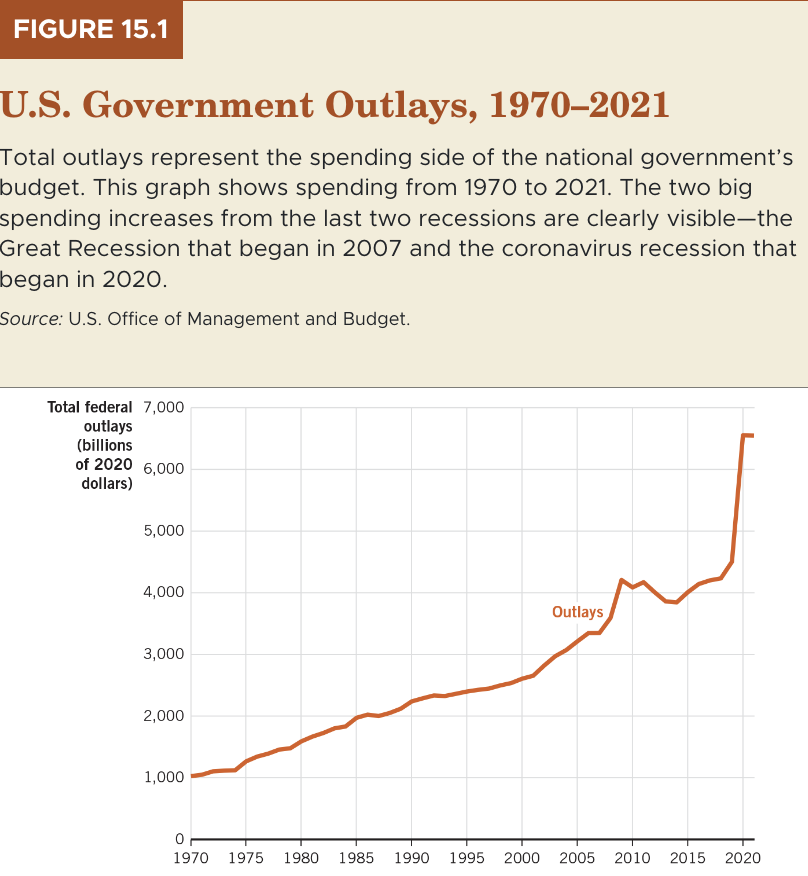
\includegraphics[scale=0.5]{images/Figure 15.1.png} 
\end{center}

\begin{center}
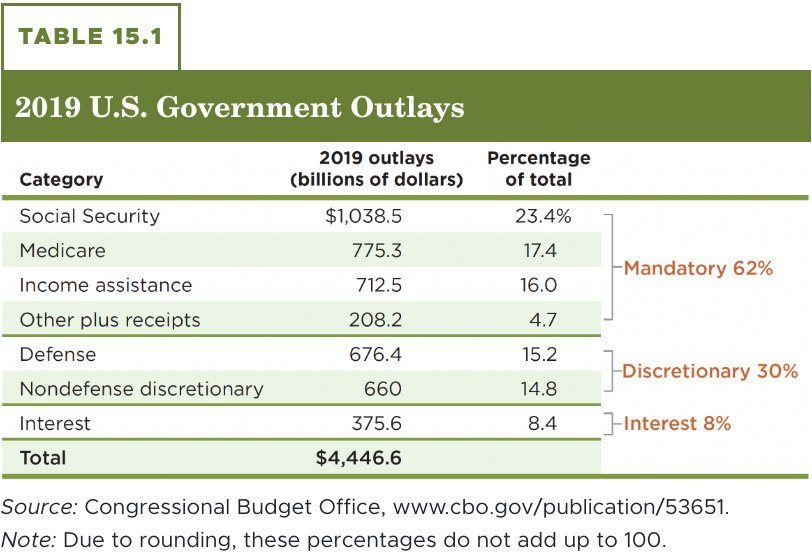
\includegraphics[scale=0.5]{images/Table 15.1.png}
\end{center}
\textbf{Discretionary outlays} are subject to adjustment during the annual budget process; examples of discretionary spending include monies for bridges and roads, payments to government workers, and defense spending. When you think of prominent government spending items, you likely first think of discretionary items; but in fact, discretionary spending accounts for less than one-third of the U.S government budget, which is now predominantly mandatory spending.

The final category in Table 15.1 is interest payments; these are payments made to current owners of U.S treasury bonds. For all practical purposes, these interest payments are also mandatory because they are not easy to alter, given a certain level of debt.

The distinction between mandatory and discretionary spending helps to explain the recent growth of government spending in many nations: much of the growth is in mandatory spending. Returning to Table 15.1, we see that mandatory spending constituted 63\% of the U.S federal budget in 2019; in fact, if we include interest payments as obligatory, that leaves just 30\% of the U.S budget where trimming is possible. You might remember this the next time you read or hear about budgetary negotiations: while much of the debate focuses on discretionary spending items like defense, bridges, and highways, or educational subsidies, the majority of the budget actually goes to mandatory categories.

\begin{center}
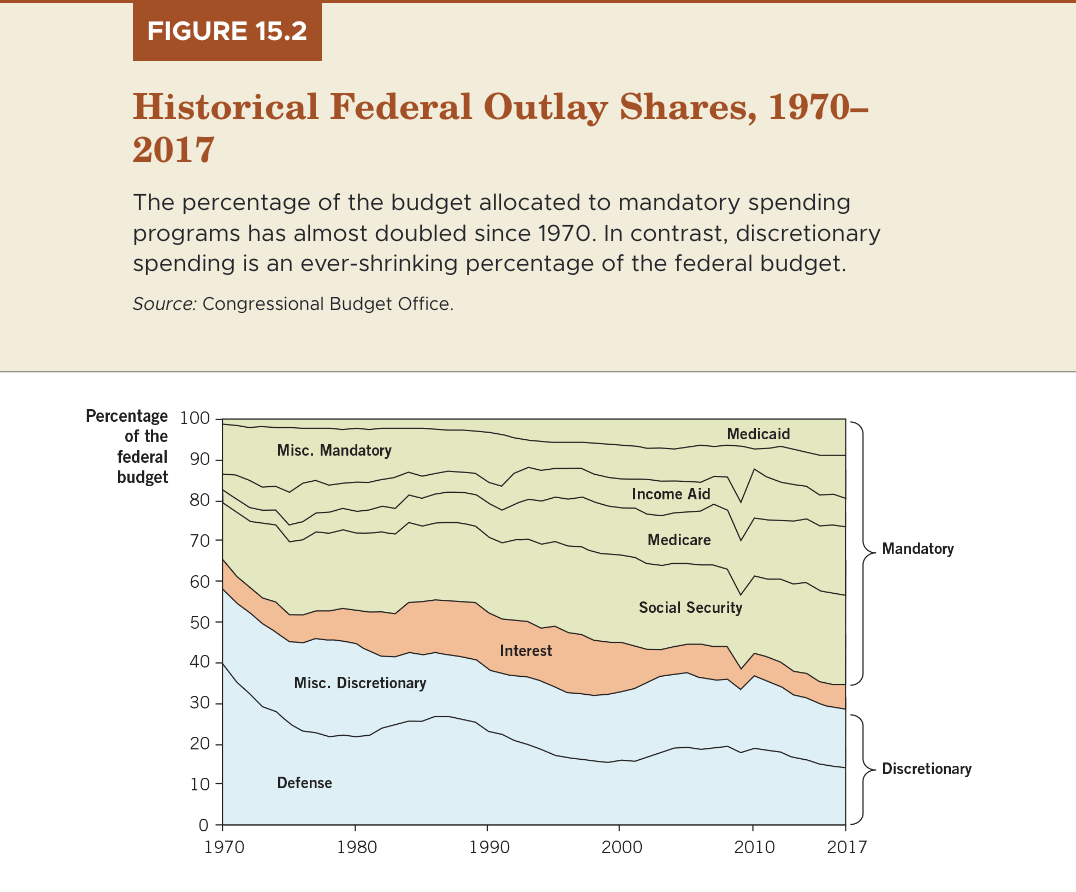
\includegraphics[scale=0.5]{images/Figure 15.2.png}
\end{center}
It wasn't always this way; Figure 15.2 plots U.S budget categories as portions of total outlays for 1970-2017. The green-shaded categories represent mandatory spending; in 1970, mandatory spending was only about one-third of the federal budget. The cause of the growth in mandatory spending over the last 50 years is both political and demographic: new mandatory programs have been added, and an aging population has led to wider eligibility for many programs, like Social Security and Medicare. Miscellaneous mandatory spending programs include unemployment compensation, income assistance (welfare), and food stamps; Medicare was added in 1966 (LBJ administration) and the expanded in 2006. By 2017, Social Security and Medicare alone accounted for 42\% of the U.S federal budget, up from just 16\% in 1970.

\subsection*{Social Security and Medicare}
In this section, we look more closely at Social Security and Medicare so we can try to understand why so many resources are devoted to these programs.

In 1935, as part of the New Deal and in the midst of the Great Depression, the U.S Congress and President Franklin Roosevelt created the Social Security program. \textbf{Social Security} is a government-administered retirement funding program; the program requires workers to contribute a portion of their earnings into the Social Security Trust Fund, with the promise that they'll receive these back (along with a modest growth rate) upon retirement. The goal of the program is to guarantee that no U.S worker retires without retirement income.

% Budget situation (FDR)

\textbf{Medicare} is a mandated federal program that funds health care for people aged 65 and older; this program was established in 1965 with the goal to providing medical insurance for all retired workers. Like Social Security, the law requires current workers to pay Medicare taxes with the promise of receiving insurance upon retirement. In 2003, Medicare was extended into reimbursements for prescription drugs for retirees as well; the total Medicare tax rate is currently 2.9\%.

Both Medicare and Social Security outlays are concentrated on the elderly population and so are greatly affected as population demographics shift. Given that these programs now account for more than 40\% of all federal outlays, we should look more closely at demographic changes before digging further into the dynamics of the federal budget.

\subsubsection*{Demographics}
Entitlement programs have come to dominate the federal budget, with Social Security and Medicare taking up ever-expanding shares. There are three underlying, and related, natural demographic reasons; first, people are living longer today than ever before, drawing post-retirement benefits for a longer period of time. In 1930, the life expectancy after age 60 was less than 14 years, limiting the length of time retirees collected Social Security benefits. Today, Americans live an average of 23 years after age 60; this is a big change from the assumptions on which the system was built.

Second, there are now far more workers retired and drawing benefits than before; to be eligible for Social Security and Medicare payments, workers pay taxes while they work. In the early years, very few were eligible for payouts, but millions were paying in; both programs naturally generated substantial tax revenue with very few outlays for many years, but with so many workers now retired...the math has changed.

Third, in addition to a normal flow of retirees, the baby boomers (people born between 1946 and 1964) are now retiring. This is a disproportionately large population cohort; thus, workers are retiring in record numbers, and this will continue for another 10-plus years. Figure 15.3 breaks down the U.S population by age, as of July 2021, with horizontal bars showing the size of the population in different age groups. This is called a population pyramid, because it would resemble an actual pyramid for a population with steady growth driven by a high population of very young children that gradually declines with age; but factor such as the baby boom and a recent decline in birthrates since 2007 have produced this funny-shaped "pyramid" that is smaller at the bottom than in the middle.

\begin{center}
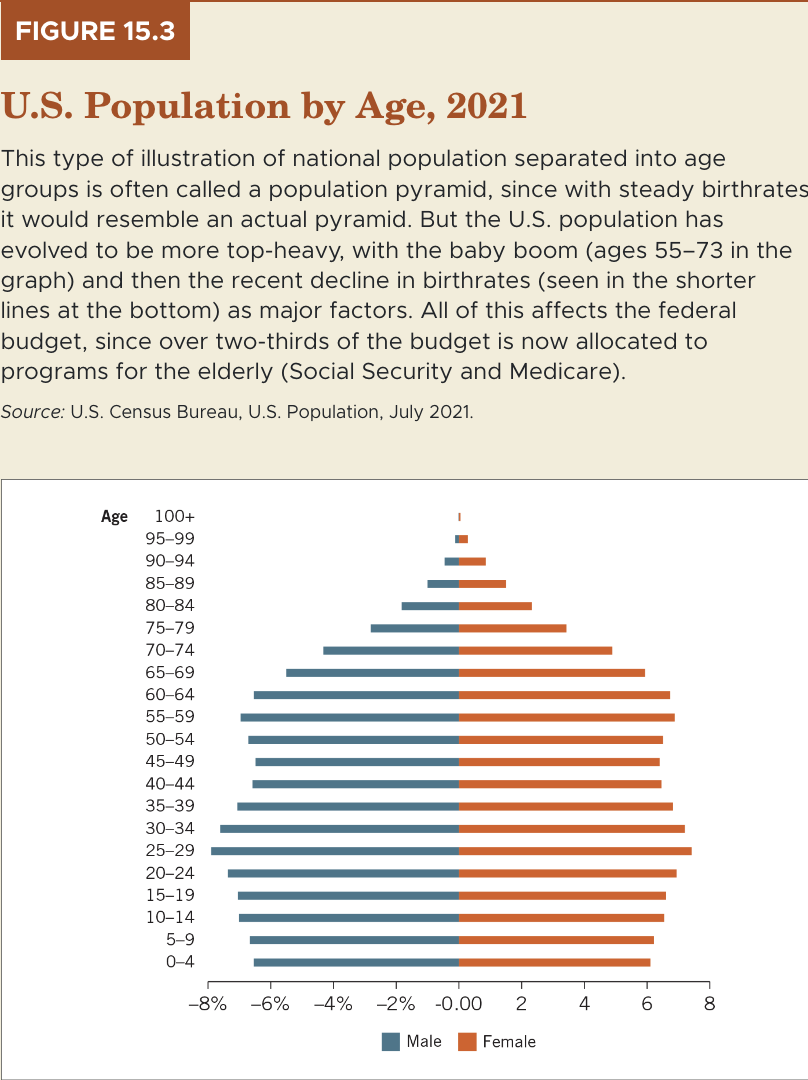
\includegraphics[scale=0.5]{images/Figure 15.3.png}
\end{center}
In the end, this matters greatly for the U.S government budget, because so many workers are now exiting the labor force, and the younger population cohorts are relatively small. This shift requires ever expanding outlays for the mandatory program. Any substantive discussion about the national debt and deficits must focus on these programs.

\subsection*{Spending and Current Fiscal Issues}
Before turning to the revenue side of the budget, we should take a close look at the recent history of U.S government outlays. Figure 15.4 shows real federal government outlays from 1990 to 2021; the first half of the graph shows relatively stable government spending, prior to our two most recent recessions, but in 2008, government outlays entered a turbulent period. We are really looking at three successive phases:
\begin{itemize}
\item \textit{1990 to 2008: Relative economic stability that required very little fiscal response}. In this period, the economy generally expanded, aside from two short recession (in 1990 and 2001).
\item \textit{2008 to 2020: The Great Recession followed by the longest economic expansion in U.S history.} The increase in outlays from 2008 to 2011 was a direct policy response to the Great Recession; government spending increased significantly at the beginning of this era. This was followed by more than ten years of economic expansion, from mid-2009 to early 2020.
\item \textit{2020 and onward: The coronavirus recession caused by the global pandemic}. The U.S government responded to the coronavirus recession with massive government spending increases. (We cover these more fully in \underline{Chapter 16}.) This is the spike you see in Figure 15.4.
\end{itemize}

\begin{center}
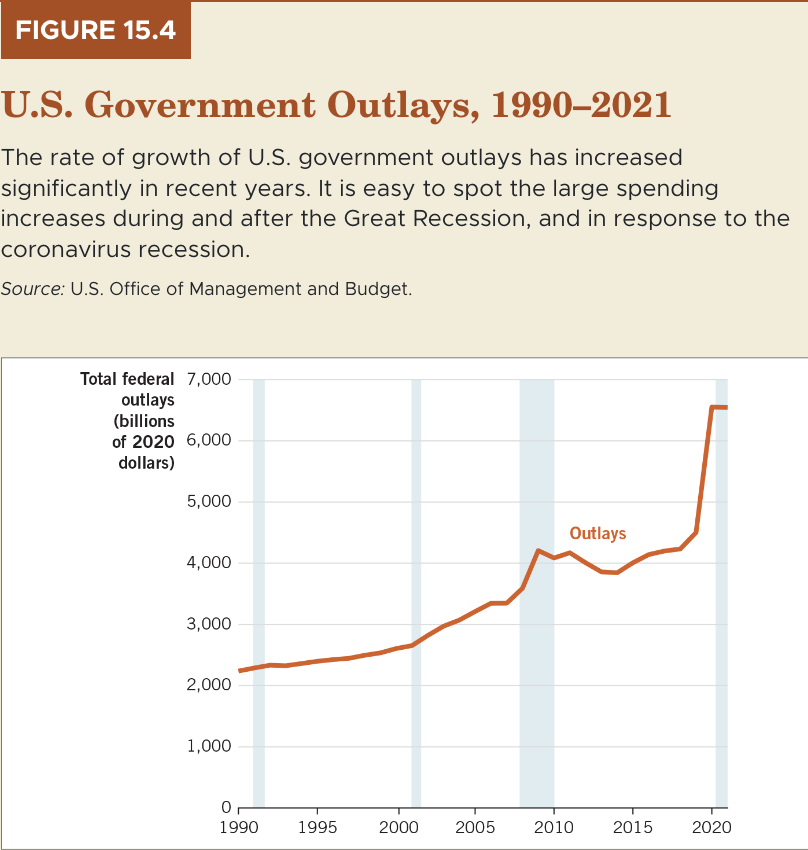
\includegraphics[scale=0.5]{images/Figure 15.4.png} 
\end{center}

\section*{How does the government tax?}
Governments raise revenues in many ways; fees assessed for government services - for example, admission fees to national parks - contribute small amounts. But almost all government revenue is raised through taxes.

No one enjoys paying taxes, but the government can't provide Social Security, Medicare, national defense, highways, and public education unless it brings in the tax revenue to pay for all those services. Yes, the government can borrow to cover the budget deficits it runs, but the government can't fund its operations entirely through borrowing. In this section, we detail the principle types of taxes the U.S government collects.

\subsection*{Sources of Tax Revenue}
Figure 15.5 shows sources of tax revenue for the U.S government in 2021; the two largest sources are individual income taxes and social insurance (Social Security and Medicare) taxes. Together, these two sources accounted for 83\% of all U.S federal tax revenue. Both of these taxes are deducted from workers' paychecks, which means that for every \$1 in federal tax revenue, \$0.83 came from taxes on individual wages.

All other major types of taxes together produced just 17\% of the federal revenue in 2021; the largest category here is corporate income taxes, which yielded \$372 billion in 2021, or 9.2\% of the total revenue. Estate and gift taxes are levied when property is gifted to others, particularly as an inheritance. Excise taxes are taxes on a particular good or commodity, such as cigarettes or gasoline; the federal excise tax on cigarettes is \$1.01 per pack, and the federal tax on gasoline is 18.4 cents per gallon. Collectively, excise taxes yielded \$75 billion in tax revenue in 2021; customs taxes are taxes on imports, and these yielded just \$80 billion in 2021.

Because income and social insurance taxes play such an outsize role, we will now discuss them in greater detail.
\begin{center}
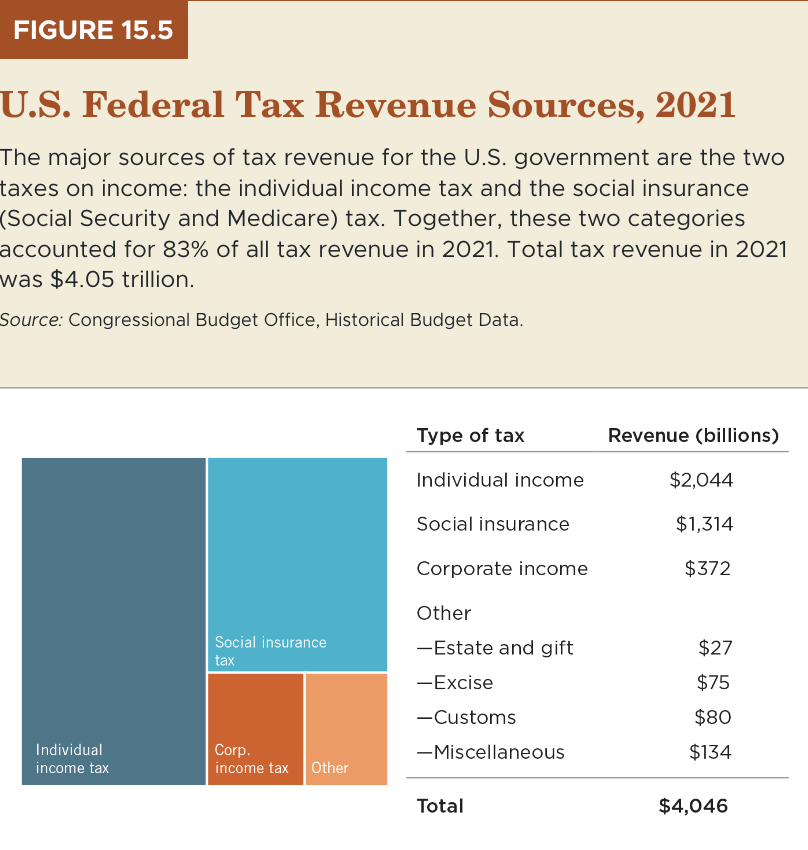
\includegraphics[scale=0.5]{images/Figure 15.5.png}
\end{center}
\subsection*{Taxes on Workers' Wages}
After you graduate from college and secure a full-time job, you'll likely earn much larger paychecks might be smaller than you expect based on your salary alone. Remember, the government pays for activities with tax revenue predominantly raised from taxes on income. Let's look more closely at the major taxes on income: the social insurance tax and individual income tax.

\subsubsection*{Social Insurance Tax}
Earlier, we discussed government outlays for Social Security and Medicare, which together account for more than 40\% of total U.S federal spending. The money spent comes from taxes on workers' paychecks; the benefits received by each retiree depend on taxes paid in during his or her working years; currently, the tax for these two programs amounts to 15.3\% of a worker's pay. This is typically split in half, with 7.65\% paid by the employee and the other 7.65\% paid by the employer; people who are self-employed pay the full 15.3\% (the Social Security portion of the tax is applicable to the first \$142,800 an individual earns). These dollars go into the Social Security and Medicare trust funds that provide income and health care assistance to retirees.

\subsubsection*{Income tax}
U.S federal income taxes are set according to a scale that increases with income levels; in a \textbf{progressive income tax system}, people with higher incomes pay  a larger percentage of their income in taxes than people with lower incomes do. Figure 15.6 shows 2021 federal income tax rates for single individuals; notice, the tax rate climbs with income level. That is what is meant when the U.S income tax system is described as "progressive"; it doesn't mean "a scheme favored by political liberals," even if liberals happen to approve.

The tax rates specified in Figure 15.6 are marginal tax rates; a \textbf{marginal tax rate} is the tax rate paid on an individual's "next dollar" of income. Consider a worker in 2021 with a salary of \$72,550; assume this worker takes the standard tax deduction of \$12,500, so taxable income is exactly \$60,000. The tax schedule in Figure 15.6 puts someone with \$60,000 of taxable income in the 22\% tax bracket; this doesn't mean that the worker pays 22\% of the entire \$60,000 in taxes. What it means is that income \textit{above \$40,525} is taxed at 22 cents on the dollar; the same worker will pay 10\% on every dollar of income up to \$9,950, and 12\% on the income between \$9,950 and \$40,525.

\begin{center}
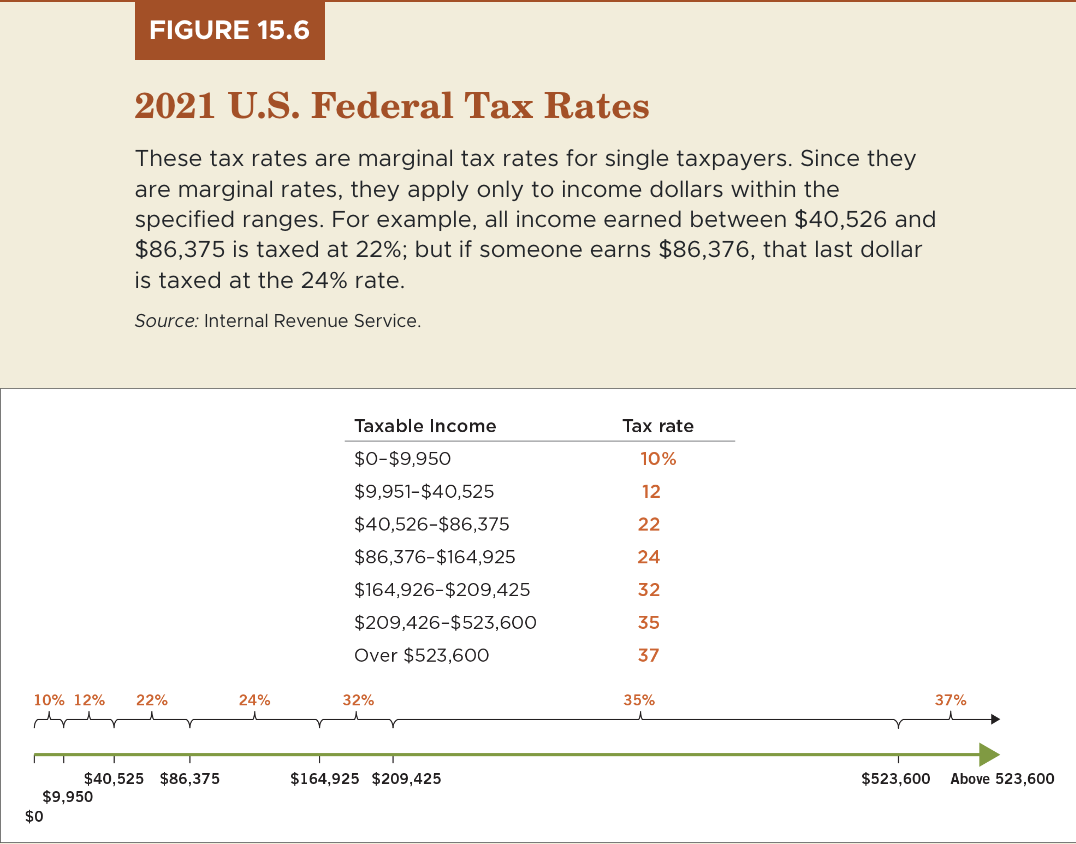
\includegraphics[scale=0.5]{images/Figure 15.6.png} 
\end{center}

\textbf{\textit{When we consider fiscal policy in Chapter 16, it will be critical to understand how income taxes are computed.}}

Let's use the rates from Figure 15.6 to compute a tax bill based on a taxable income of \$60,000; note again that three different tax rates apply: 10\% on income up to \$9,950; 12\% on income from \$9,951 to \$40,525; and 22\% on income from \$40,526 to \$60,000. The total tax bill then comes to:
\begin{center}
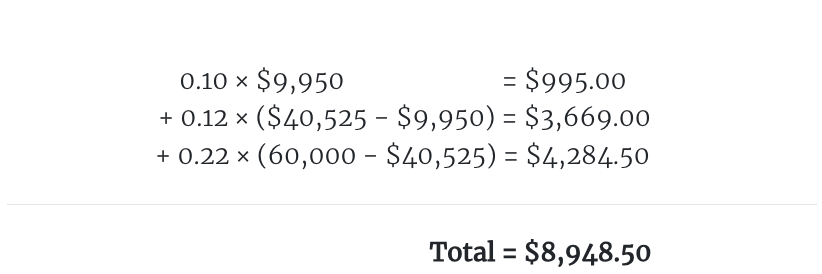
\includegraphics[scale=0.75]{images/Tax bill Example.png} 
\end{center}
Therefore, \$60,00 in taxable income will accrue a federal income tax bill of \$8,948.50, which is 14.9\% of the taxable income (\$60,000). This 14.9\% is the taxpayer's average tax rate; an \textbf{average tax rate} is the total tax paid divided by taxable income. Notice that the average tax rate is below the marginal tax rate (22\%); this is generally the case in a progressive tax system, because the marginal tax rate applies to the last few dollars taxed, rather than all income.

\subsection*{Historical income tax rates}
Although income taxes seem like a fact of life, the U.S income tax is only about 110 years old. Prior to 1913, there was no income tax in the United States; most tax revenues were generated by taxes on imports (tariffs), but import taxes were declining. So the government introduced income taxes as another source of revenue; the original income tax in the United States was similar to the current tax system, in that the rates were progressive. But it was very different in terms of the actual tax rates: the highest marginal rate in 1913 was just 6\%, and that rate applied only to income greater than \$500,000 - over \$11 million in today's dollars; very few people were earning that kind of income in 1913. (Not many people earn that kind of income now, for that matter.)

Once income taxes were in place, marginal tax rates rose quickly; by 1918, in fact, the top marginal rate was up yo 77\%. This rate applied only to income over \$2 million, but it meant that every dollar earned beyond \$2 million netted only 23 cents to the income earner, after taxes. Figure 15.7 plots the top marginal income tax rates in the United States from 1913 to 2021. Note that while this figure shows only the top rate, it is a good indicator of the general level of rates over time.

We can point to many important dates in the evolution of U.S income tax rates; during the 1930s, in the midst of the Great Depression, with income levels plunging, income tax revenues naturally fell. President Hoover and Roosevelt, attempting to balance the federal budget, pressed Congress to increase top marginal rates to 80\%. As you might expect, this did not help an already struggling economy; later, in 1963, with top marginal rates at their historically highest level (over 90\%), President Kennedy pushed for tax rate reductions that dropped the top rate to 70\%. In the 1980s, President Reagan led the push to lower marginal tax rates even further; by the end of the decade, the top marginal rate was just 28\%. In 1993, President Clinton proposed higher rates, and the top rate rose to 39.6\%; President George W. Bush pushed through a temporary decrease in this top rate in 2003, and the lower rate of 35\% persisted for 10 years, before the top rate returned to 39.6\% in 2013. Finally, in December 2017, the top marginal tax rate fell to 37\% as part of the Tax Cuts and Jobs Act of 2017, which we discuss later in this chapter. Over the course of a century, there was a great deal of fluctuation in marginal rates; going forward, it is not likely that top rates will ever return to the levels witnessed prior to 1980.

\begin{center}
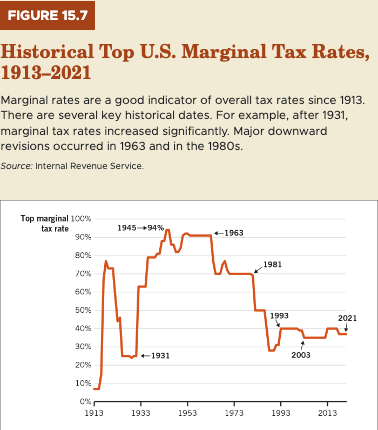
\includegraphics[scale=0.5]{images/Figure 15.7.png}
\end{center}
\subsection*{How are taxes distributed across income levels in the United States?}
In a progressive income tax system, tax rates rise with income; this means that high income taxpayers pay more than low-income ones, not only in absolute terms (which would be true even with a flat tax) but as a percentage of income, and so they end up paying the lion's share of total taxes. This is certainly true in the United States; Figure 15.8 plots total U.S federal tax shares paid by different income groups (by household) in the United States from 1980 to 2018. These are the shares of all federal taxes paid, including income taxes, Social Security and Medicare taxes, excise taxes, and corporate taxes; the top line represents the share of taxes paid by the wealthiest 20\% of households. You can see that this share has been hovering around 70\% of all federal taxes paid; in contrast, the 20\% of U.S households with the lowest incomes paid zero net federal taxes paid in 2018.(In this group, the positive taxes paid by some households were offset by tax credits paid to other households.) In fact, in 2018, the top 1\% (not pictured) of all households paid about the same amount of federal taxes as the entire bottom 80\% combined (30\%).

\begin{center}
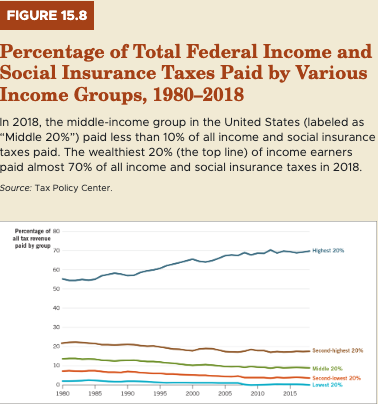
\includegraphics[scale=0.7]{images/Figure 15.8.png}
\end{center}

\section*{What are budget deficits?}
We are now ready to bring both sides of the budget together; doing so enables us to examine the differences between spending and revenue. In this section, we define budget deficits and debt, and also consider these in historical context.

\subsection*{Deficits}
A \textbf{budget deficit} occurs when the government outlays exceed revenue in a given time period, usually a year. Panel (a) of Figure 15.9 plots U.S budget outlays and revenues from 1970 to 2021, in billions of 2020 dollars. Outlays are displayed in orange and revenues in blue; you can see that outlays generally exceed revenue. The biggest difference came in 2020, when outlays were \$6.55 trillion and revenue was just \$3.42 trillion; the difference, \$3.13 trillion, was the deficit for 2020.

It possible to for the government to have a \textbf{budget surplus}, which occurs when revenue exceeds outlays; the most recent U.S federal surpluses came in four years from 1998 to 2001. Panel (b) of Figure 15.9 graphs the budget balance from 1970 to 2021; when budget is in deficit, the balance is negative, when the budget is in surplus, the balance is positive.

\begin{center}
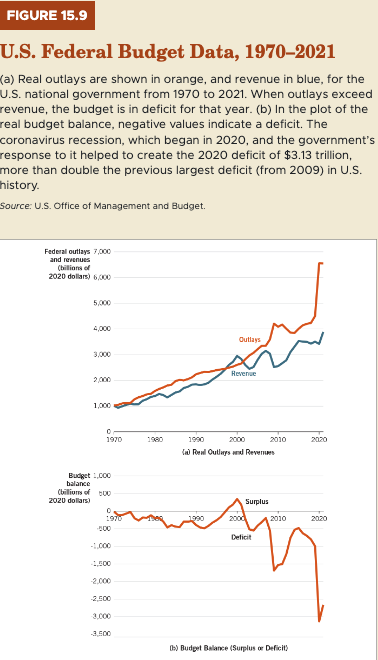
\includegraphics[scale=0.4]{images/Figure 15.9.png}
\end{center}
The 2020 deficit of \$3.13 trillion is the largest in U.S history - larger in real dollar terms than the deficits generated during World War II in the 1940s; but dollar values for government budget figures, even in real dollars, are misleading over the long run, because the population and the size of the economy change. To control for both population and economic growth, economists often look at the budget deficit as a percentage of GDP; dividing budget data by GDP scales it to the size of the economy. Figure 15.10 shows the U.S federal outlays and revenue, both as a fraction of GDP, from 1970 to 2021; over the entire period, outlays averaged 20.4\% of GDP and revenues averaged 17.0\% of GDP. These averages are shown as dashed lines in the figure; you can view these long-run averages as a benchmark for future budgets. Both outlays and revenues currently lie outside their long-run averages.

The blue vertical bars in Figure 15.10 indicate economic recessions; when a recession hits, tax revenue, which is largely tied with income, declines. In addition, for reasons we cover in the next chapter, government outlays often increase during the recessions. Together these two results cause deficits to increase during recessions.

When the budget is in deficit, the government must borrow funds to pay for the difference between outlays and revenue. In Chapter 10, we introduced U.S Treasury bonds as important financial assets in the loanable funds market. Now we can understand how those bonds originate: when tax revenues fall short of outlays, the government sells Treasury bonds to cover the difference. The aftereffects of COVID-19 and the government's response to it were still playing out in the summer of 2022.

\begin{center}
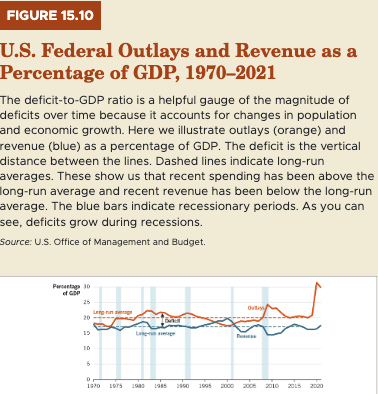
\includegraphics[scale=0.5]{images/Figure 15.10.png}
\end{center}
\subsection*{Deficits versus Debt}
In your personal budget, it might happen that your spending (outlays) in a given month exceeds your income; in other words, you find you have a deficit. You might rely on funds from parents or grandparents to make up the difference, but this money counts either as income (if it's a gift) or as a loan (if you have to repay it). Often, you will have to borrow, perhaps by using a credit card; a loan, whether it is from a friend or relative, or a credit card company, is a debt that must be paid.

It's easy to confuse the terms "deficit" and "debt"; a deficit is a shortfall in revenue for a particular year's budget. A \textbf{debt} is the total of all accumulated and unpaid budget deficits; consider your tuition bill over the course of your time in college. If you borrow \$5,000 to help pay for your first year in college, that is your first-year deficit; if you borrow another \$5,000 for your second year, you have a \$5,000 deficit each year and your debt grows to \$10,000. This is the same way that national debt grows; any year in which there is a budget deficit leads to a larger national debt.

Figure 15.11 shows the U.S national debt (in real terms) from 1990 to 2021; notice that we distinguish total national debt and debt held by the public. The difference between these is debt owned internally by one of the many branches of the U.S government. Sometimes, a given federal agency purchases Treasury bonds; for example, as part of its mandate to control the money supply, the Federal Reserve typically holds billions of dollars' worth of Treasury securities. Thus, it is helpful to distinguish total government debt that is not also owned by the government itself, and this is the public held portion. Figure 15.11 indicates that both measures have risen in recent years, a result of the large budget deficits.

\begin{center}
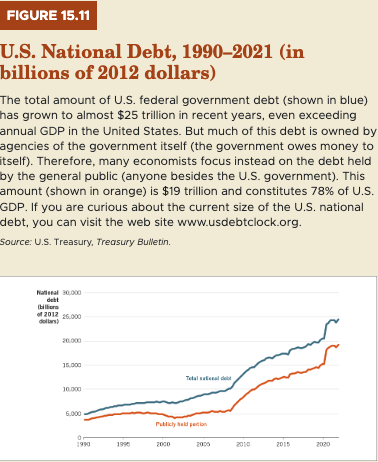
\includegraphics[scale=0.5]{images/Figure 15.11.png}
\end{center}
While the U.S national debt is historically large, relative to the size of the economy it is still smaller than that of many other nations, including many wealthy ones. Figure 15.12 shows publicly held debt-to-GDP ratios for several nations in 2020; the United States comes in at 128\%, but Japan's ratio is over 260\%.

\begin{center}
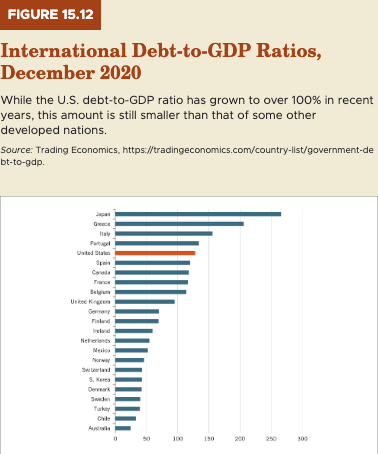
\includegraphics[scale=0.5]{images/Figure 15.12.png} 
\end{center}
\begin{center}
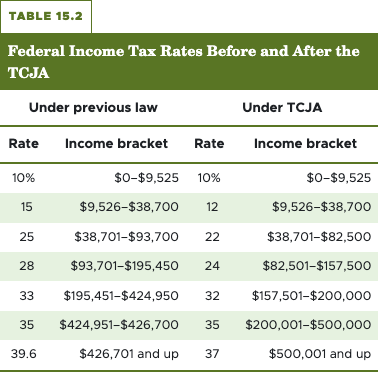
\includegraphics[scale=0.5]{images/Table 15.2.png} 
\end{center}

\subsection*{Foreign Ownership of U.S Federal Debt}
As we saw in Chapter 10, many people are concerned about foreign ownership of U.S debt; the concern stems from a fear that foreigners who own U.S debt can control the country politically and economically. However, according to the U.S Treasury, as of 2018, about 70\% of U.S national debt was held domestically, and just 30\% internationally. China, Japan, Brazil, and the United Kingdom are the major foreign holders of U.S debt.

Figure 15.13 shows foreign and domestic ownership of total real U.S debt from 1990 to 2018; during this period, total national debt grew from \$6 trillion to over \$26 trillion (in 2019 dollars). However, domestic investors and U.S government agencies were the purchasers of most of the new debt. The portion of U.S government debt that is foreign owned is less than 30\%.

While this foreign ownership of U.S government debt is troubling for many Americans, it is important to recognize the benefits of foreign funds to the U.S loanable funds market. As we discussed in Chapter 10, foreign lending increases the supply of loanable funds in the United States, helping reduce interest rates. Lower interest rates mean that firms and governments in the United States can borrow at lower cost and thereby increase investment and hire more workers, and ultimately increase future production. Furthermore, the increase in foreign ownership is a natural by-product of emerging foreign economies - as they get wealthier, they buy more U.S treasury bonds.

\begin{center}
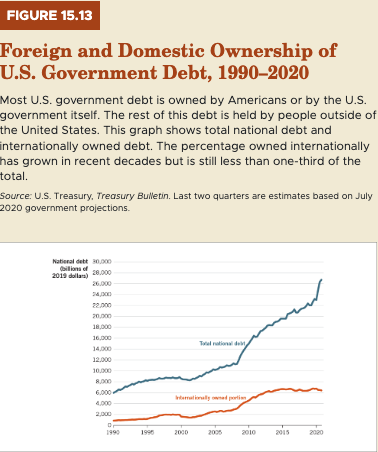
\includegraphics[scale=0.5]{images/Figure 15.13.png}
\end{center}

\section*{Conclusion}
We started this chapter with the observation that governments rarely balance their budgets; we then looked more closely at government outlays and revenues. This chapter lays the groundwork for us to examine fiscal policy in Chapter 16; much of the debt and deficits we observed are a direct result of government budgetary maneuvers to affect the macroeconomy. Going forward, we now understand the institutions of fiscal policy; in Chapter 16, we'll learn about the economic theories that support fiscal policy.
\end{document}
